\documentclass[tikz,border=0pt]{standalone}
\usepackage[american]{circuitikz}
\usetikzlibrary{arrows.meta,calc,positioning,decorations.pathmorphing,patterns}
\definecolor{zyloTeal}{HTML}{174A5B}
\definecolor{zyloTealTwo}{HTML}{246B7A}
\definecolor{zyloInk}{HTML}{1F2933}
\definecolor{zyloSoft}{HTML}{EAF4F4}
\definecolor{zyloPaper}{HTML}{F8FAFB}
\definecolor{zyloLine}{HTML}{44606B}
\definecolor{zyloOrange}{HTML}{D97706}
\begin{document}
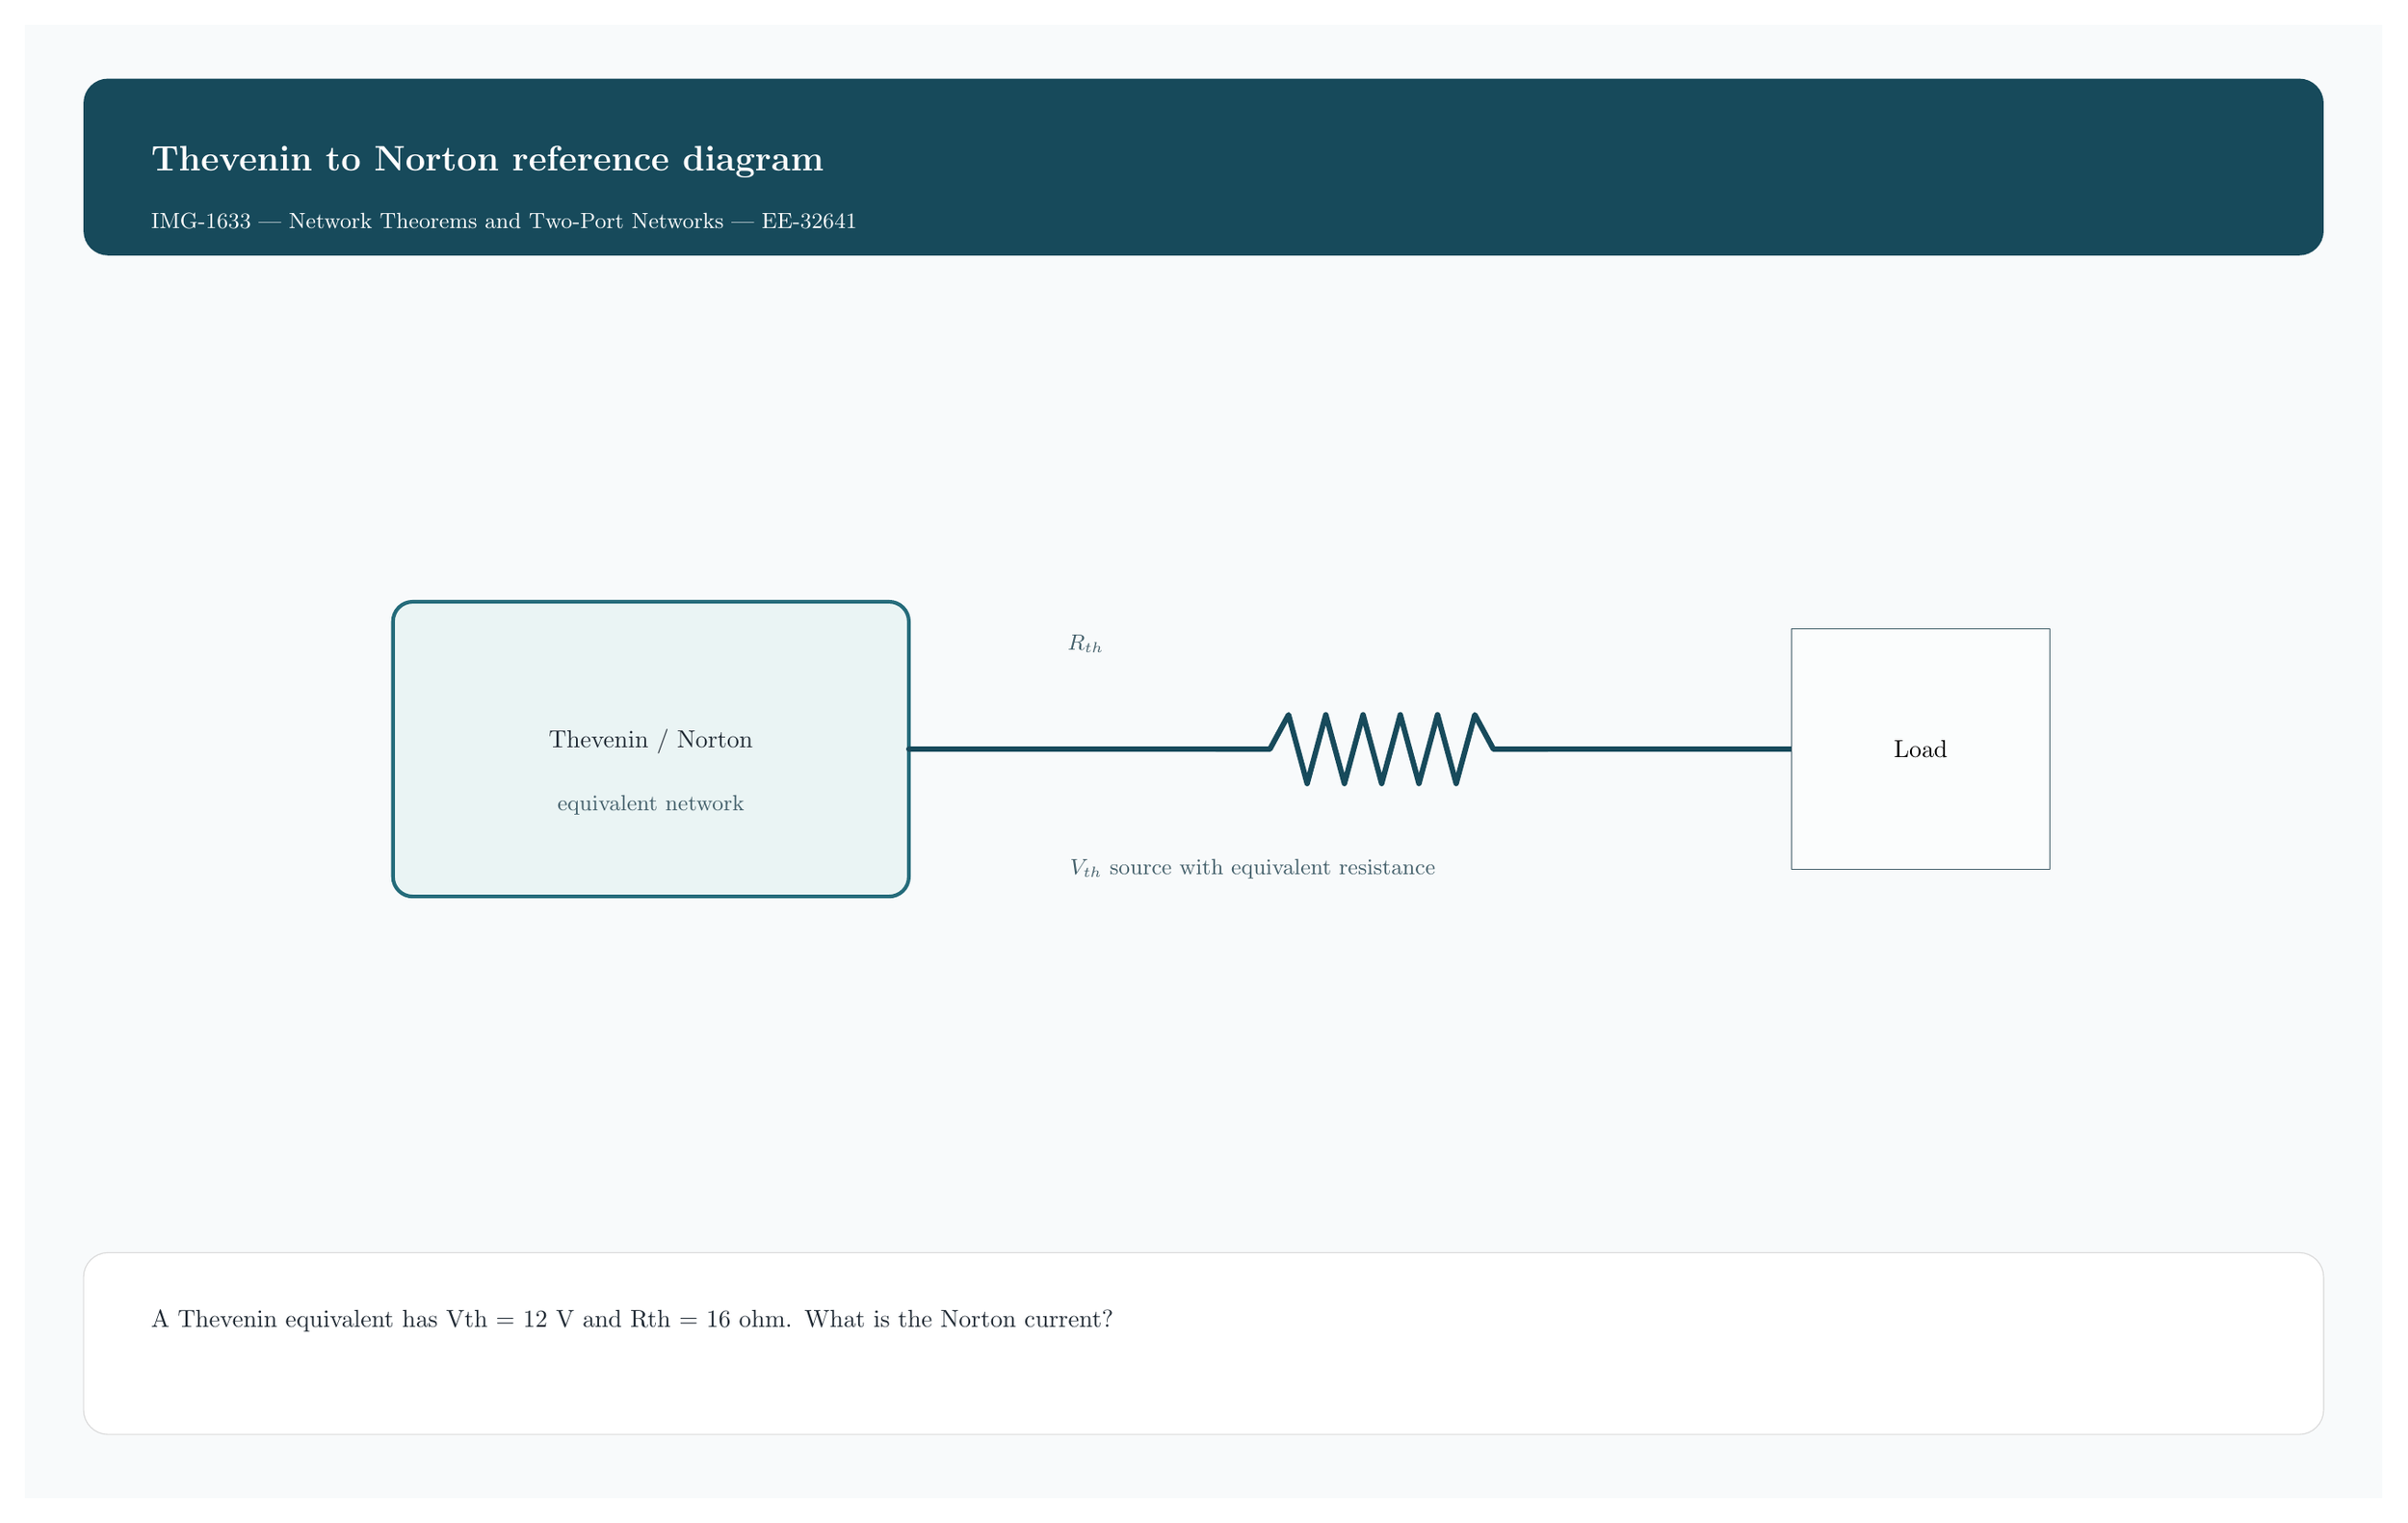
\begin{tikzpicture}[x=1pt,y=-1pt,>=Latex,line cap=round,line join=round]
\path[fill=zyloPaper] (0,0) rectangle (960,600);
\path[fill=zyloTeal,rounded corners=10pt] (24,22) rectangle (936,94);
\node[anchor=west,text=white,font=\bfseries\Large] at (48,56) {Thevenin to Norton reference diagram};
\node[anchor=west,text=white!82,font=\small] at (48,80) {IMG-1633 | Network Theorems and Two-Port Networks | EE-32641};
\tikzset{wire/.style={draw=zyloTeal,line width=2.2pt},thinwire/.style={draw=zyloLine,line width=1.35pt},accent/.style={draw=zyloOrange,line width=2.2pt},box/.style={draw=zyloTealTwo,fill=zyloSoft,line width=1.5pt,rounded corners=8pt}}
\node[box,minimum width=210pt,minimum height=120pt] at (255,295) {};
\node[text=zyloInk] at (255,292) {Thevenin / Norton}; \node[font=\small,text=zyloLine] at (255,318) {equivalent network};
\draw[wire] (360,295) -- (485,295);
\draw[wire] (485,295) -- (507,295) -- (507,295) -- (514.583,281) -- (522.167,309) -- (529.75,281) -- (537.333,309) -- (544.917,281) -- (552.5,309) -- (560.083,281) -- (567.667,309) -- (575.25,281) -- (582.833,309) -- (590.417,281) -- (598,295) -- (620,295);
\draw[wire] (620,295) -- (720,295);
\node[draw=zyloLine,fill=white!80!zyloSoft,minimum width=105pt,minimum height=98pt] at (772,295) {Load};
\node[font=\small,text=zyloLine] at (432,252) {$R_{th}$}; \node[font=\small,text=zyloLine] at (500,344) {$V_{th}$ source with equivalent resistance};
\path[draw=black!15,fill=white,rounded corners=10pt] (24,500) rectangle (936,574);
\node[anchor=west,text width=860pt,align=left,text=zyloInk,font=\normalsize] at (48,528) {A Thevenin equivalent has Vth = 12 V and Rth = 16 ohm. What is the Norton current?};
\end{tikzpicture}
\end{document}
